\section{Traitement des images et création des matrices pour l'algorithme d'apprentissage}

\subsection{Présentation des images}

À chaque sujet correspond une image de dimension (182, 218, 182) (voir~\autoref{fig:IRM}).
Les images sont regroupées en un seul fichier qui correspond donc à un volume 4D (3 dimensions d'une image plus une dimension pour les sujets).
En plus de ces images, on peut utiliser une étape supplémentaire de traitement appelée squelettisation (voir~\autoref{fig:IRM_skel}) qui permet de réduire les images à un ensemble de courbes.

\begin{figure}[htpb]
	\centering
	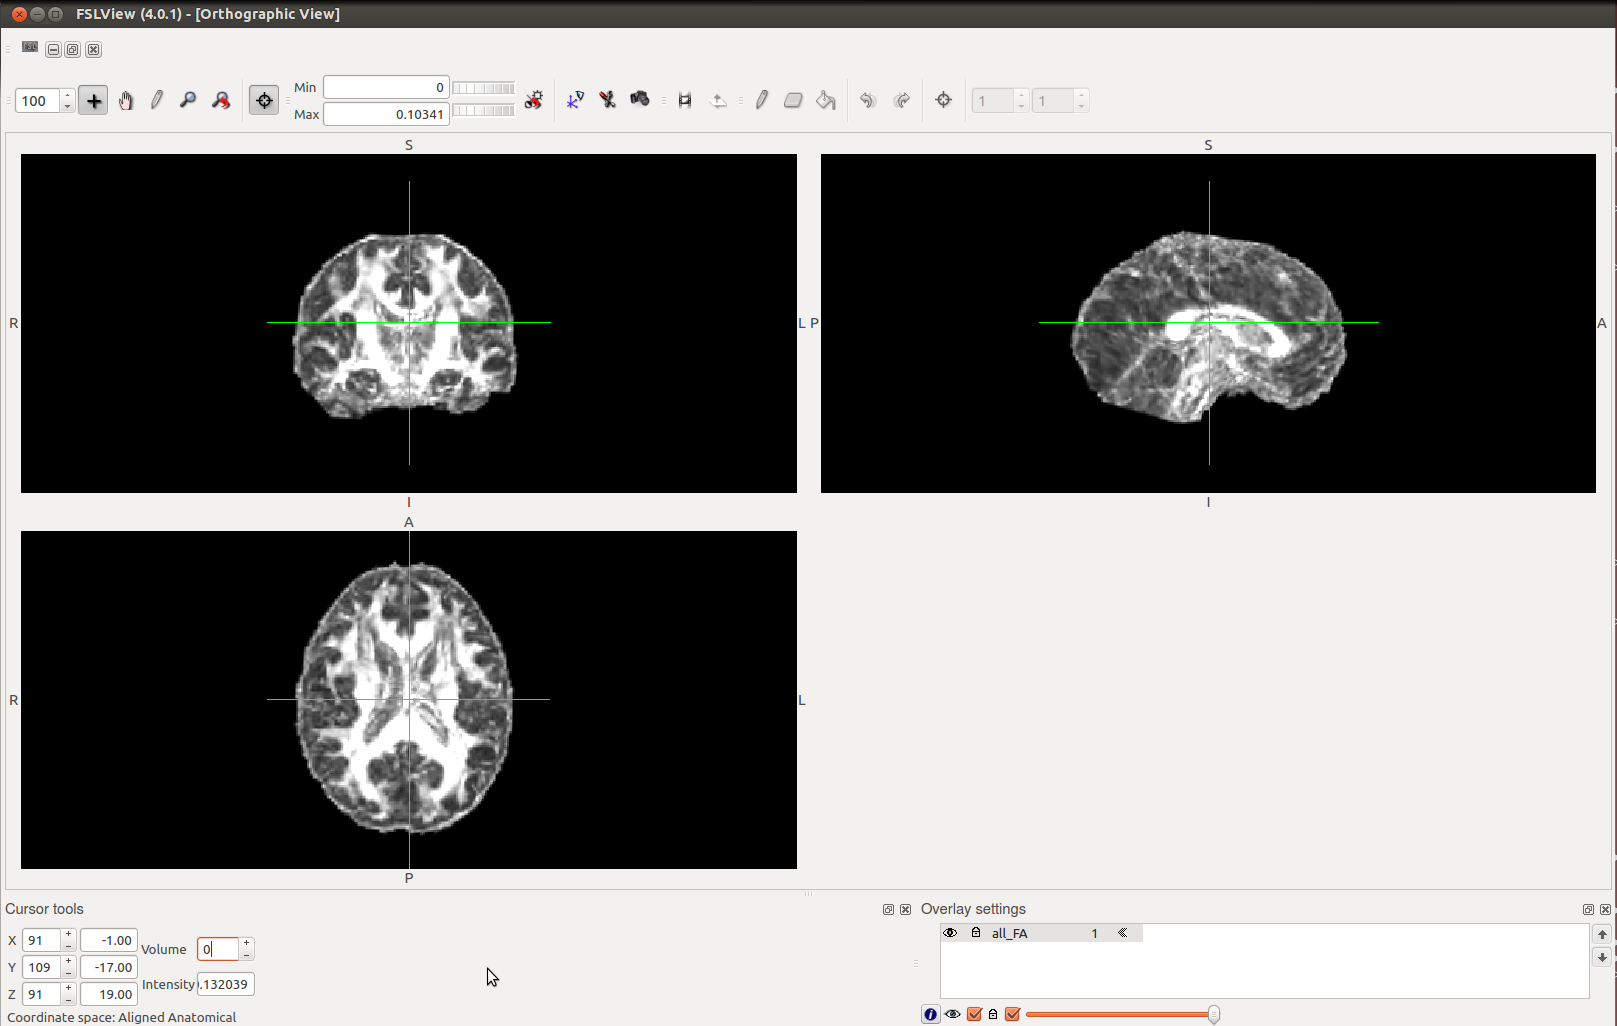
\includegraphics[scale = 0.5]{images/example_dwi}
	\caption{IRM de diffusion.}
	\label{fig:IRM}
\end{figure}

\begin{figure}[htpb]
	\centering
	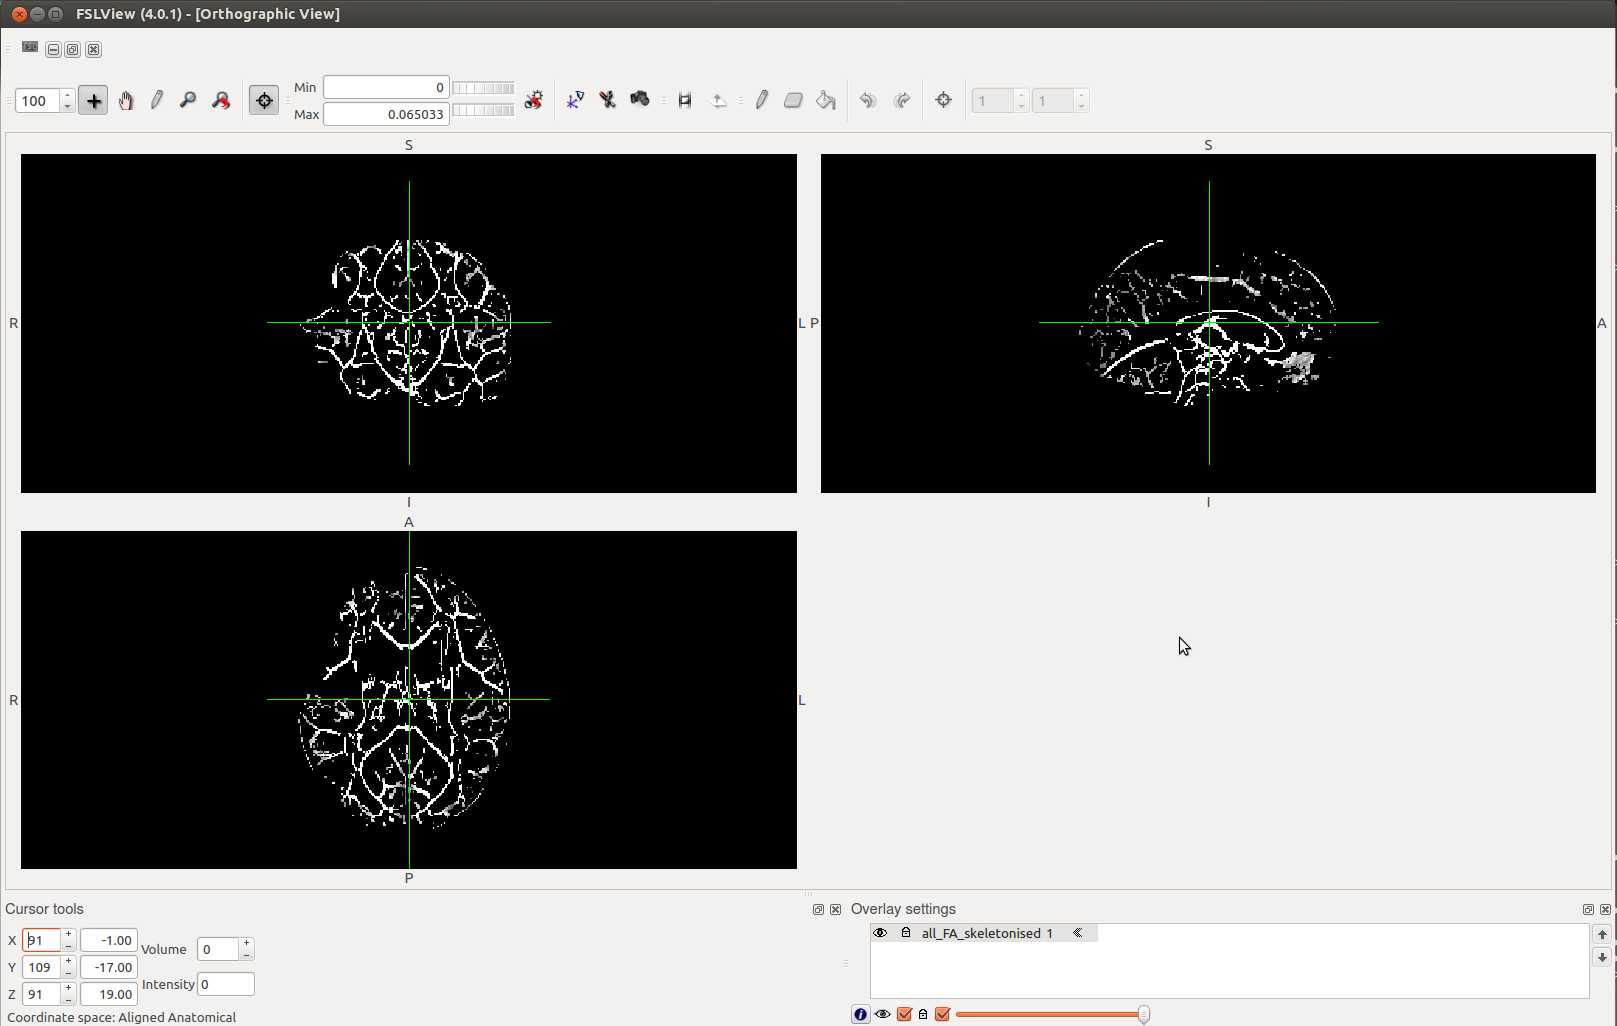
\includegraphics[scale = 0.5]{images/example_dwi_skel}
	\caption{IRM de diffusion squelettisé.}
	\label{fig:IRM_skel}
\end{figure}


\subsection{Création du masque}

Chaque image fait environ deux millions de voxels. Nous allons appliquer un masque afin de réduire le nombre de voxel et ainsi focaliser notre analyse sur une plus petite partie du cerveau. Cela nous permettra d'éliminer une grande partie des voxels qui ne nous intéressent pas. 
Ce masque (voir~\autoref{fig:masque}) sera réalisé selon les images de base avec un certain seuil suivi d'un peaufinage basé sur un atlas qui va nous permettre de sélectionner des régions du cerveau qui ne sont pas révélatrices dans notre cas. 

Dans le cas des images squelettisées (voir~\autoref{fig:masque squelétisé}), nous créons le masque sur la base de ces images. 

Dans le cas du masque tronqué (voir~\autoref{fig:mask tronqué}), nous suivons les mêmes étapes ci-dessus, suivi de l'élimination des zones du cerveau non-informatives (l'arrière du cerveau).



\begin{figure}[h]
	\centering
	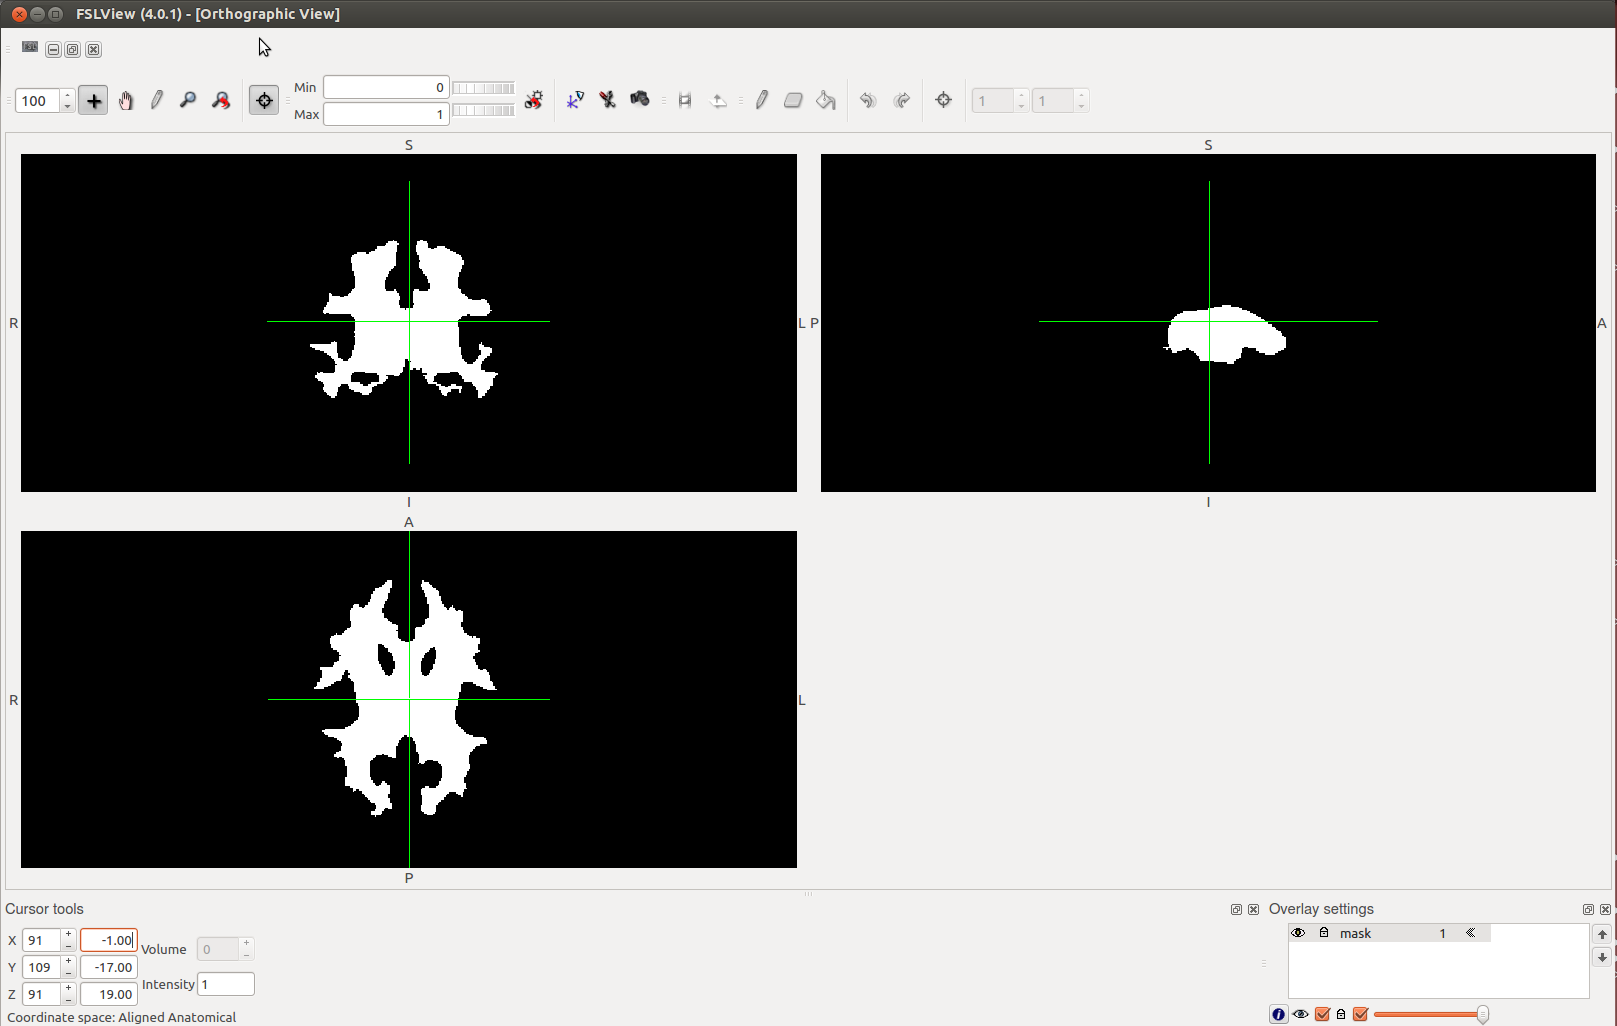
\includegraphics[scale = 0.5]{images/mask}
	\caption{Masque sans modification.}
	\label{fig:masque}
\end{figure}

\begin{figure}[h]
	\centering
	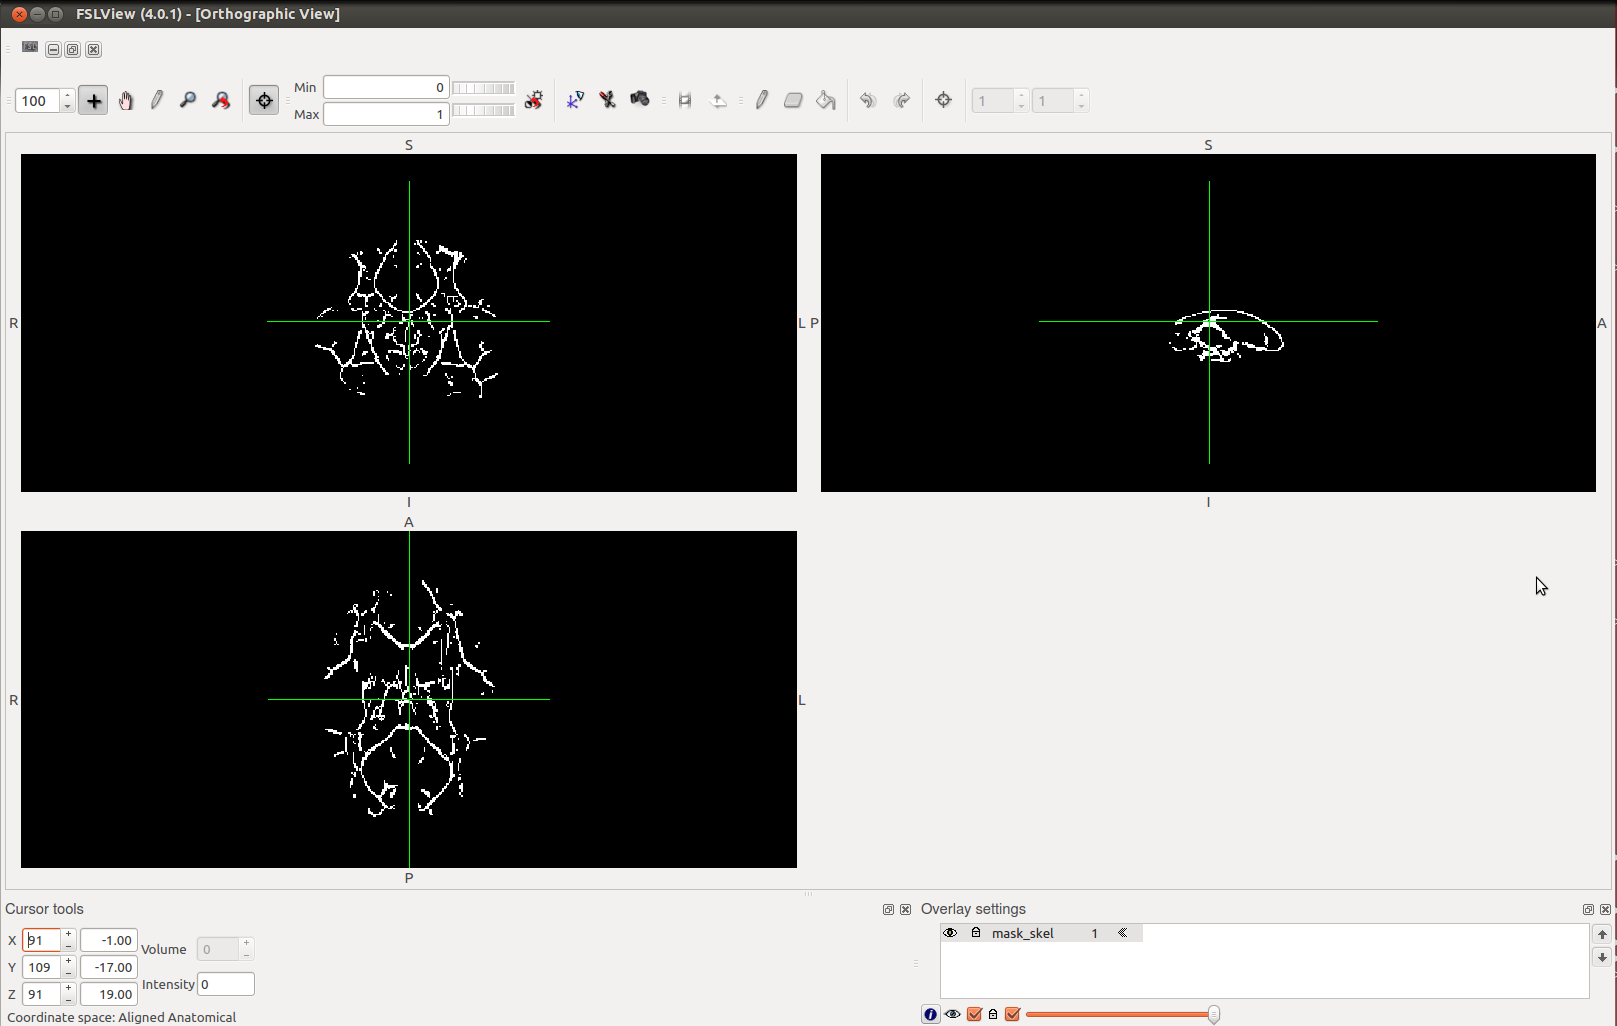
\includegraphics[scale = 0.5]{images/mask_skel}
	\caption{Masque réalisé à partir des images squelétisées.}
	\label{fig:masque squelétisé}
\end{figure}
  	
\begin{figure}[t]
	\centering
	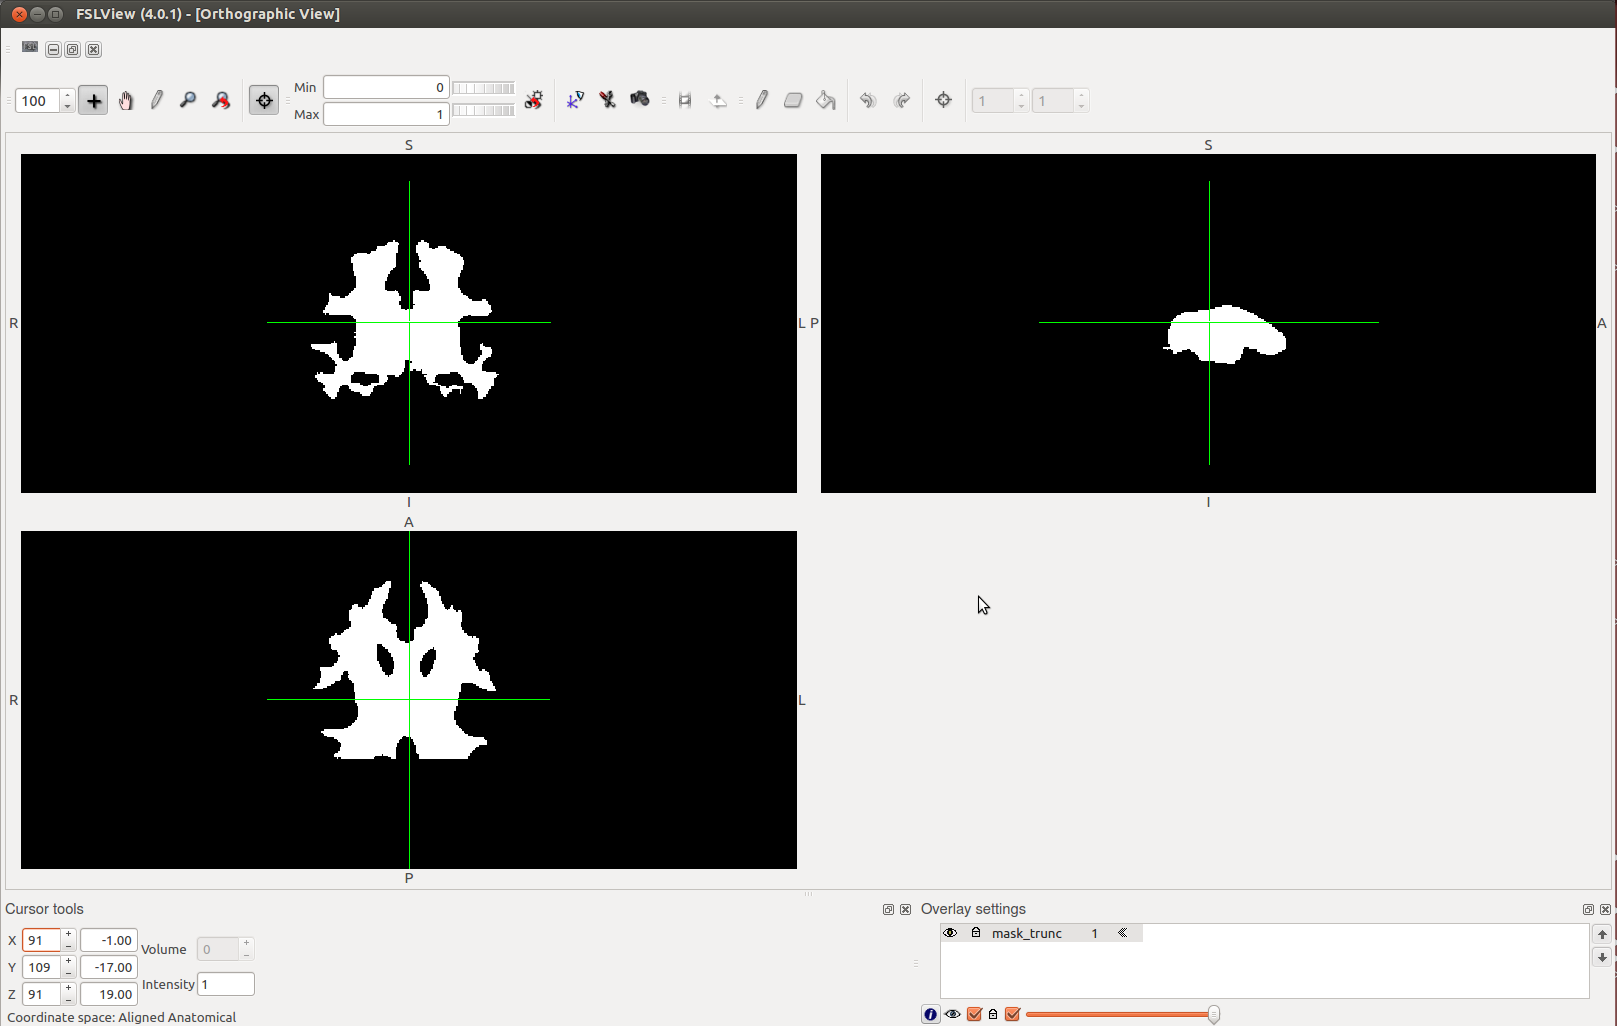
\includegraphics[scale = 0.5]{images/mask_trunk}
	\caption{Masque tronqué.}
	\label{fig:mask tronqué}
\end{figure}


\subsection{Application du masque}

Chaque image 3D est transformée en un vecteur ligne appelé \textit{vecteur d'image}.
De même, le masque est transformé en vecteur ligne.
Ce masque est utilisé pour sélectionner des éléments du vecteur.

Ainsi, nous obtenons une matrice de vecteurs où chaque ligne correspond à un sujet où le nombre de colonne correspond au nombre de voxels du masque.

Cette matrice sera ensuite centrée et réduite afin d'être normalisée. 
Cette démarche est commune à toutes les hypothèses. 

\subsection{Ajout des covariables}

Suite à la création de cette matrice, nous ajoutons des colonnes de covariables. Ces covariables sont des données cliniques qui ne seront pas pénalisées lors du calcul de prédiction. Les covariables sont le sexe des sujets et leur âge auquel a été pris l'image. 
L'âge sera centré et réduit mais pas le sexe qui sera codé en binaire (1, -1) ou le 1 correspond aux femmes et -1 les hommes. 
Ces deux colonnes sont ensuite ajoutées a la matrice X. 
Une dernière colonne est ajoutée, qui joue le rôle de l'ordonnée à l'origine et qui a pour but de diminuer l'effet biaisé (équilibrage de la classification des sujets)

Dans le cas de l'hypothèse 3, une covariable va être ajoutée, celle des sites où a été prise l'IRM. Il s'agit du \textit{Dummy Coding}, c'est à dire transformée une colonne contenant plusieurs informations qualitatives en n colonnes, une pour chaque valeur différente. 

Une autre matrice est créée, celle des Y qui correspond à l'état clinique des sujets (sain ou malade). Cette matrice est commune a toutes les hypothèses. 

Ces deux matrices seront enregistrées dans deux fichiers différents et seront utilisées lors du calcul d'apprentissage et de prédiction.


Suite à cela, nous lançons les calculs de prédiction sur un cluster. 


